\documentclass{article}
\usepackage{JML}
\usepackage{amsfonts}
\usepackage{graphicx}
\usepackage{dsfont}
\usepackage[left=1in,right=1in]{geometry}
\title{The BLMP: Constrained Linear Predictors}
\setlength\parskip{5pt}
\setlength\parindent{0pt}
\def\llangle{\left\langle}
\def\rrangle{\right\rangle}
\newcommand\E[1]{\llangle #1 \rrangle}

\newcounter{version}
\setcounter{version}{0}
\newcommand\attempt[1]{\stepcounter{version} \section*{Version \theversion: #1}}

\begin{document}
	\maketitle

	This document is a neatened up version of various attempts towards deriving the Best Linear Monotonic Predictor. 

	\section*{The Goal}
		Consider a second order random process $X$, such that at each value of $t \in \mathbb{R}$, we have a random variable $X_t$. 

		We may randomly sample this vector at $n$ points, gaining a vector $\vec{T} = (t_1,t_2,t_3,\hdots)$ of itmes at which the samples were made, and $\vec{X} = (X_{t_i})$. Strictly speaking these are both random variables in and of themselves, up until the moment that we `realise' them. We can index into these vectors using the the integer $0 \leq i < n$, and we assume without loss of generality that the samples are sorted in time, such that $t_i < t_{i+1} \forall i$.

		We wish to find a predictor, $\hat{X}_t$, which will predict the value of $X_t$ at a given value of $t$, subject to two further conditions:
		\begin{itemize}
			\item The only thing we `know' (or are willing to \textit{ansatz}) about $X_t$ is the second moment kernel (a generalisation of the covariance):
			$$ \E{X_t X_s} = k(t,s)$$
			\item Our predictor should be linear, such that:
			$$\hat{X}_t = \vec{a}_t \cdot \vec{X}$$
		\end{itemize}
		We again reiterate that $X_t, \vec{X}$ and $\hat{X}_t$ are - strictly speaking - random variables until we make them into real numbers at the moment we wish to actually make a prediction. $\vec{a}_t$ is a real $n$-tuple, which takes on different values at each value of $t$.

		These are the ingredients of the standard BLP. We extend this by further adding the knowledge that the underlying process -- and hence the predictions -- should be monotonic in $t$, such that $X_{t_1} \leq  X_{t_2}$ if $t_1 \leq t_2$.
	\attempt{The Standard BLP}

		We first begin by deriving the normal Best Linear Predictor, since it useful to have the derivation as a starting point for our more advanced methods. 

		Our definition of `best' will be the standard Mean Squaure Error, averaged across the random variables (and not $t$, as I was first confused by). 
		
		\begin{spalign}
			\mathcal{L} & = \sum_{t \in T} \mathcal{M}_t
			\\
			& = \sum_{t \in T} \langle (X_t - \hat{X}_t)^2 \rangle \label{E:GlobalLagrangian}
		\end{spalign}
		Here the sum runs across a set $T$ of chosen `prediction points' where we wish to estimate the value. However, we note that the problem of predicting $X_t$ is wholly separable; meaning that it is possible to infer the value of each $t$ independently, rather than as a whole. Maximising each $\mathcal{M}_t$ individually will maximise $\mathcal{L}$.
		\begin{spalign}
			\mathcal{M}_t(\vec{a}_t) & = \E{\left(X_t - \vec{a} \cdot \vec{X}\right)^2}
			\\
			& = \E{X_t^2} - 2  \cdot \E{X_t \vec{a}\cdot \vec{X}} + \E{(\vec{a}\cdot\vec{X})^2} \label{E:NastyEq}
		\end{spalign}
		Although we have now assembled our cost function in terms of our variable of interest $(\vec{a}_t$), we are in something of a bind	, since we know nothing about the behaviour of $X_t$; not its mean or variance. However, we are willing to conjure up a second moment kernel of some kind, noting that this gives us the following definitions:
		\begin{align}
			\left[\vec{k}_t \right]_i & = k(t,t_i) = \E{X_t X_{t_i}}
			\\
			K_{ij} & = k(t_i, t_j) = \E{X_{t_i} X_{t_j}}
		\end{align}
		\def\a{\vec{a}_t}
		Noting that - as a real-valued quantity - $\vec{a}$ passes through the expectation values, we therefore find that \eref{E:NastyEq} simplifies to:
		\begin{equation}
			\mathcal{M}_t = \E{X_t^2} - 2 \vec{k}_t \cdot \a + \a \cdot \left( K \a\right) \label{E:BLP_Lagrangian}
		\end{equation}
		This rearrangement is useful to us as it has rewritten our cost function in terms of a constant-valued (and hence irrelevant) unknown quantity, and functions of the second moment kernel which we are willing to guess at. Computing the derivatives, we find:
		\begin{spalign}
			\pdiv{\mathcal{M}_t}{\a} = -2 \vec{k}_t + 2 K\a \LLR \a^\text{best} = K^{-1} \vec{k}_t
		\end{spalign}
		Since $K$ is symmetric, $K^{-1}$ is also symmetric, and hence we can write the best linear predictor as:
		\begin{equation}
			\hat{X}_t = \vec{k}_t \cdot \left( K^{-1} \vec{X} \right)
		\end{equation}
		Since $K$ is a function only of $\vec{X}$, the quantity $K^{-1} \vec{X}$ can be precomputed, hence allowing for efficient computation of $\hat{X}$ at all desired values of $t$. 

		We also recall that since the problem was totally separable, we could make an inference on a set $t \in T$, and then subsquently expand our predictions to another set $t \in T^\prime$ wihtout recomputing the original predictions. 

	\attempt{The Peicewise-Local Constraint}

		We now begin imposing the monotonicity constraints: that $\hat{X}_{t_i} \leq \hat{X}_{t_{i+1}}$, where we have assumed w.l.g. that both $\vec{T}$ and $t \in T$ are sorted to themselves be monotonically increasing. If this is not the case, then the first step is to sort the values such that this is the case. 
		
		As the end point of chain, we find that $\hat{X}_{t_0}$ is unconstrained, and hence the Lagrangian is unaltered from the original form of \eref{E:BLP_Lagrangian}
		\begin{equation}
			\hat{X}_{t_0} = \vec{k}_{t_0} \cdot \left( K^{-1} \vec{X} \right)
		\end{equation}

		The next steps in the sequence contain a `slack variable' in the Lagrangian:
		\begin{spalign}
			\mathcal{M}_{t_{i > 0}} & = \E{X_t^2} - 2 \vec{k}_t \cdot \a + \a \cdot \left( K \a\right) + \lambda \left( \hat{X}_{t_i} - \hat{X}_{t_{i-1}} - s^2 \right)
		\end{spalign}
		Here $\lambda, s \in \mathbb{R}$, and hence this acts as a constraint enforcing $\hat{X}_{t_i} = \hat{X}_{t_{i-1}} + s^2$, which enforces the monotonicity for all values of $s$. However, we note that we are not actually interested in the value of $s$, since this is an \textit{inequality} constraint; we are merely interested in ensuring that $\hat{X}_{t_i} > \hat{X}_{t_{i+1}}$, not controlling \textit{how much greater} it is. 

		We can therefore make use of the Karush-Kuhn-Tucker (KKT) conditions, and assert that when $s \neq 0$, $\lambda = 0$, and when $\lambda \neq 0, s = 0$: i.e. $\lambda$ is only non-zero when the constraint is active (i.e. the solution would otherwise break monotonicity).

		Optimising this w.r.t. $\a$ (and making the assumption that $\a \neq f(\vec{a}_{t-1})$) gives:
		\begin{spalign}
			\pdiv{\mathcal{M}_t}{\a} &= -2 \vec{k}_t + 2 K\a + \lambda \vec{X} 
			\\
			\a &= K^{-1} \left(\vec{k}_t - \frac{\lambda}{2} \vec{X} \right)
			\\
			\hat{X}_t & = \vec{k}_t \cdot K^{-1} \vec{X} - \frac{\lambda}{2} \vec{X} \cdot K \vec{X} 
		\end{spalign}
		If the monotonicity constraint is met, and the original BLP solution was monotonic between $t_i$ and $t_{i-1}$, then the KKT conditions tell us that $\lambda = 0$ and we recover the original solution. If, however, the solution is non-monotonic, then $\lambda \neq 0$, $s = 0$, and we find that:
		\begin{spalign}
			\lambda & = 2\frac{\vec{k}_t \cdot K^{-1} \vec{X} - \hat{X}_{t_{i-1}}}{\vec{X} \cdot K \vec{X} }
		\end{spalign}
		All of which is to say, that a locally-enforced monotonic (LEM-) BLP takes the form:
		\begin{equation}
			\hat{X}_{t_i} = \begin{cases} \vec{k}_{t_i} \cdot K^{-1} \vec{X} & \text{if this is } \geq \hat{X}_{t_{i-1}}
				\\
				\hat{X}_{t_{i-1}} & \text{else}
			\end{cases}
		\end{equation}
		In short; whenever the LEM-BLP is identical to the BLO, until the BLP breaks monotonicity, at which point the LEM-BLP predicts a horizontal line, until the BLP rises above this line again.


	\attempt{The BLMP}

		We note that in deriving the LEM-BLP, we made a crucial assumption - namely that we could maintain the separable nature of the solutions, and that minimising $\mathcal{M}_t$ individually would minimise the global Lagrangian $\mathcal{L}$ of \eref{E:GlobalLagrangian}. This assumption meant that we could take the derivative of $\mathcal{M}_t$ w.r.t. $\vec{a}_{t_i}$ whilst treating it as a constant w.r.t. $\vec{a}_{t_{i-1}}$.

		In a globally-enforced predictor- the Best Linear Monotonic Predictor (BLMP) - this should not be the case; our definition of `best' should be global, not local. 

		Hence, in this attempt, we try to minimise $\mathcal{L}$ simultaneously over the entire set of prediction points $t\in T$. This has the important corollary that should we wish to predict a new time $s \notin T$, we would have to re-run the entire global analysis on the set $t \in \{s, T\}$, which might have a drastically different output. 

		We therefore perform a change of coordinates - rather than trying to predict the random variables $\{\hat{X}_t\}$, we are trying to predict the random variables $\{z_i\}$, which are related to $\hat{X}$ through the following transform:
		\begin{spalign}
			\hat{X}_{t_0} & = z_0
			\\
			\hat{X}_{t_{i>0}} & = \hat{X}_{t_{i-1}} + e^{z_i}
		\end{spalign}
		This transformation imposes no constraints on $\hat{X}$ asides from monotonicity, and is therefore totally general on the space of BLMPs. The random variables $\{z_i\}$ are totally unconstrained on $\mathbb{R}$.

		For notational convenience, we relabel the states $X_{t_i}$ as $X_i$, and so the sum $t \in T$ runs over $0 \leq i < N$, and package $\{z_i\}$ into a vector $\vec{z}$. We can then write:
		\begin{spalign}
			\hat{X}_i & = S_i(\vec{z})
			\\
			&  = z_0 + \sum_{j=1}^i e^{z_j}
		\end{spalign}
		
		The constrained Lagrangian is therefore:

		\begin{equation}
			\mathcal{L} = \left(\sum_{i  = 0}^{N-1} \E{X_i^2} + \vec{a}_i \cdot K \vec{a}_i - 2 \vec{k}_i \cdot \vec{a}_i\right) - \mu_0 \left( \vec{a}_0\cdot\vec{X} - z_0\right) - \sum_{i = 1}^{N-1} \mu_j \left(\left(\vec{a}_i - \vec{a}_{i-1}\right)\cdot \vec{X} - e^{z_i}\right)
		\end{equation}

		We might wonder why we have left things in terms of $\vec{a}$, when we have already stated our intention to analyse this problem in $\vec{z}$-space. Why go around the houses, when we could just write $\vec{a}_i \cdot \vec{X} = S_i$? Firstly, this is because the dot product is not invertible -- and more importantly, it is because we spent quite some time in te BLP derivation writing the Lagrangian in a way that removed our reliance on computing $\E{X_t}$, which we achieved through $\vec{a}$. 

		Our goal is therefore to find a way to express $\vec{a}_i$ in terms of $S_i$, such that we can rewrite our Lagrangian in terms of functions only of $\vec{z}$.
		\def\ai{\vec{a}_i}
		\def\vi{\vec{v}_i}
		\def\wi{\vec{w}}
		
		The Lagrangian is optimised at a value of $\ai$:
		\begin{spalign}
			\ai &= K_i^{-1} \left(\vec{k}_i - \frac{\Delta_i}{2} \vec{X} \right)
			\\
			\Delta_i &= \begin{cases} \mu_{i+1} - \mu_i & \text{if } 0 \leq j < N-1
				\\
				-\mu_{N-1} & \text{else} \end{cases}
		\end{spalign}
		We then write:
		\begin{align}
			\ai & = \vi - \frac{\Delta_i}{2} \wi
			\\
			\vi & = K^{-1} \vec{k}_i
			\\
			\wi & = K^{-1} \vec{X}
		\end{align}
		Since $\ai \cdot \vec{X} = S_i$, by definition, we therefore have:
		\begin{spalign}
			S_i & = A_i - \frac{\Delta_i}{2} B
			\\
			A_i & = \vi \cdot \vec{X}
			\\
			B & = \wi \cdot \vec{X}
		\end{spalign}
		We note that $A_i$ is simply the BLP predictor, and $B$ (like $\wi$) is a quantity which depends only on $\vec{X}$. Therefore, we find that:
		\begin{equation}
			\vec{a}_i = \vi + \frac{S_i - A_i}{B} \wi
		\end{equation}
		Putting this back into the Lagrangian, we find that  our constraint terms vanish since they are automatically satisfied by our reparameterisation, and:

		\begin{spalign}
			\mathcal{L}(\vec{z}) & = \left(\sum_{i  = 0}^{N-1} \E{X_i^2} + \vec{a}_i(\vec{z}) \cdot K \vec{a}_i(\vec{z}) - 2 \vec{k}_i \cdot \vec{a}_i(\vec{z})\right)
			\\
			& \vdots
			\\
			& = \sum_{i  = 0}^{N-1}  \text{constant in terms of $\vec{z}$} + \frac{1}{B} \left( S_i^2 - S_i \left(A_i + \vec{k}_i \cdot \wi \right)\right)
			\\
			& = \sum_{i  = 0}^{N-1}  \text{constant in terms of $\vec{z}$} + \frac{1}{B} \left( S_i^2 - 2 S_i A_i \right)
		\end{spalign}
		Where the last equality follows from the fact that $A_i = \vec{X} \cdot \left(K^{-1} \vec{k}_i\right) = \vec{k}_i \cdot \left(K^{-1} \vec{X} \right) = \wi \cdot \vec{k}_i$, due to the symmetry of $K$. Hence, the derivative with respect to $z_j$ is:
		\begin{align}
			\pdiv{\mathcal{L}}{z_j} = \frac{2}{B}\sum_i \left( S_i - A_i \right) \times \pdiv{S_i}{z_j}
		\end{align}
		Recalling the definition of $S_i$, we find:
		\begin{spalign}
			\pdiv{S_i}{z_j} & = \pdiv{}{z_j} \left( z_0 + \sum_{k = 1}^{i} e^{z_k} \right)
			\\
			& = \begin{cases} 1 & \text{if } j = 0
				\\
				e^{z_j} & \text{if } 0 < j \leq i
				\\
				0 & \text{else} \end{cases}
		\end{spalign}
		Hence:
		\begin{spalign}
			\pdiv{\mathcal{L}}{z_0} & = \frac{2}{B}\sum_{j=0}^{N-1}\left(S_j - A_j \right)
			%  \times \begin{cases}
			% 	1 & i = 0
			% 	 \\
			% 	e^{z_j} & 0 < j \leq N-1
			% \end{cases}
			\\
			\pdiv{\mathcal{L}}{z_{i>0}} & = \frac{2}{B}e^{z_i} \sum_{j=i}^{N-1}\left(S_j - A_j \right)
		\end{spalign}

		We note that the gradient is obviously zero if $A_j = S_j$, and we note that $A_j$ is identically equal to the BLP prediction. This therefore demonstrates that in the cases where the BLP is already monotonic, the BLMP predictions will be identical. 

		If the BLP is not identical, then it is impossible to set $S_j = A_j$, as $S_j$ is constrained to be monotonically increasing in $t_j$, and so the solutions differ.
	
	\attempt{Shifted BLMPs}

		One of the known quirks of a BLP is that for small kernel smoothing distances (i.e. a small `memory'), the prediction will revert to a value of 0

		\subsubsection*{The toy problem}

			Consider the simple dataset $t = \{0,5,10\}$, $\vec{X}_t = (3,6,10)$, and suppose a Gaussian Kernel with a smoothing length of 1. The standard BLP for this problem would take the following form:
			\begin{align}
					K &= \sigma^2 \begin{pmatrix}
					1	& e^{-12.5}	& e^{-50}
					\\
					e^{-12.5} & 	1 & e^{-12.5}
					\\
					e^{-50} & e^{-12.5} & 1	
				\end{pmatrix}
				\\
				K^{-1}  &= \frac{1}{\sigma^2 (1 - e^{-25})^2} \begin{pmatrix}
					\frac{1}{e^{-25} +1}	& -e^{-25/2}	& \frac{1}{1 + e^{25}}
					\\
					-e^{-25/2} & 	1 + e^{-50} & -e^{-25/2}
					\\
					\frac{1}{1 + e^{25}} & -e^{-25/2} & \frac{1}{e^{-25} +1}
				\end{pmatrix} 
				\\
				\vec{k}_t &= \sigma^2\begin{pmatrix}
					\exp\left(-\frac{t^2}{2}\right)
					\\
					\exp\left(-\frac{(t-5)^2}{2}\right)
					\\
					\exp\left(-\frac{(t-10)^2}{2}\right)
				\end{pmatrix}
				\\
				\hat{X}_t &= 3\exp\left(-\frac{t^2}{2}\right) + 6 \exp\left(-\frac{(t-5)^2}{2}\right) + 10 \exp\left(-\frac{(t-10)^2}{2}\right) + O(10^{-6})
			\end{align}
			\begin{figure}
				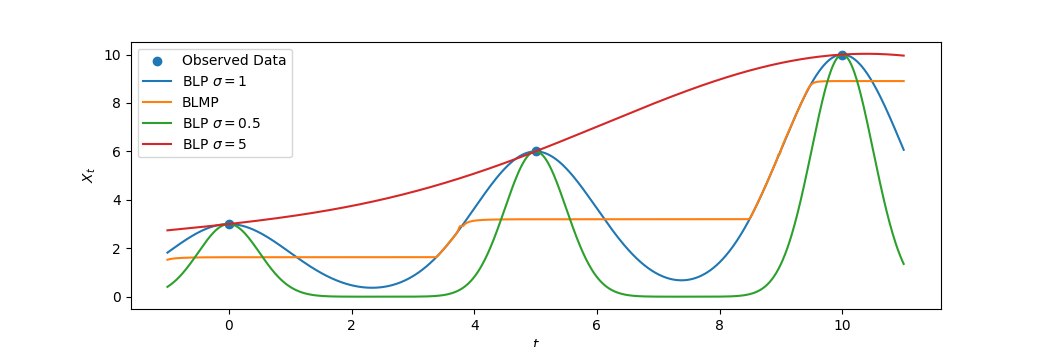
\includegraphics[width=\linewidth,keepaspectratio=true]{Figs/zeroReversion.png}
				\caption{A plot of the toy problem and the resulting BLP and BLMP predictions}\label{F:ZeroRevert}
			\end{figure}
			A plot of this predictor (and its BLMP equivalent) is shown in Fig. \ref{F:ZeroRevert}. We can see that when the prediction points are a significant way away from the sampled points, then the data reverts back to a value of zero -- a state of affairs which is obviously worsened when the smoothing distance is shortened. The BLMP struggles to cope with the resulting up-and-down predictions, and tries to strike a middle course which places its predictions nowhere near the datapoints themselves. 

			We might naturally say that this was a fault of choosing a smoothing length which was far too small for our data -- and we can see that when $\sigma = 5$, this problem vanishes and we produce a smooth (monotonic) prediction with no reversion to zero. 

			However, there might be cases where -- due to stochastic noise, perhaps -- we do end up with a gap in our data larger than our smoothing distance, in which case we would still end up with a reversion to zero -- and we might wish to prevent this from happening in some (vaguely) statistically rigorous way. 
			
		\subsubsection*{The Normal Solution}
			The usual solution that is invoked is to ensure that the data reverts to the \textit{mean}, rather than to zero. This is achieved by performing a transformation on the data, $\vec{X}^\prime = \vec{X} - \mu_X$ (where a vector-scalar subtraction is understodo to occur element-wise), and then computing the BLP on $\vec{X}^\prime$:
			\begin{equation}
				\hat{X} = \mu_X + \vec{k}_t \cdot K^{-1} \left( \vec{X} - \mu_X\right)
			\end{equation} 
			Since the mean $\langle X_t \rangle$ is inaccessible (the entire exercise of $\vec{k}$ and $K$ was to sidestep this), it is common to use the sample mean. The result of this is shown in Fig. \ref{F:MeanRevert}, showing a much more reasonable prediction than before. 
			
			However, we note that using the sample mean has its own problems: in Fig \ref{F:MeanRevert_More} we show the same predictor, but evaluated on an extended dataset with samples densly packed around $t = 10$. This biases the mean strongly upwards, and therefore drastically alters the prediction at $t = < 0$, for example, despite no new data being added here. 

			\begin{figure}
				\includegraphics[width=\linewidth,keepaspectratio=true]{Figs/meanReversion.png}
				\caption{As with Fig. \ref{F:ZeroRevert}, but with mean-reversion.}\label{F:MeanRevert}
			\end{figure}

			\begin{figure}
				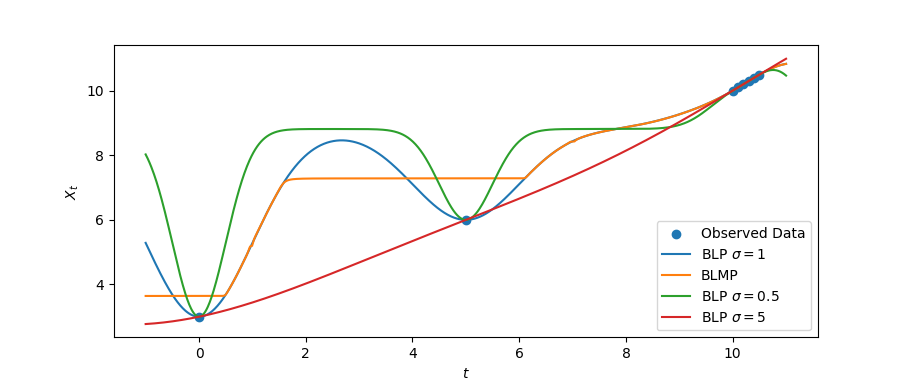
\includegraphics[width=\linewidth,keepaspectratio=true]{Figs/MeanReversion_Additional}
				\caption{As with Fig. \ref{F:MeanRevert}, but with additional data added around $t=10$, showing how altering the mean biases the prediction.}\label{F:MeanRevert_More}
			\end{figure}
		\subsubsection*{Formalising the Shifts}

			As far as I have seen, the subtraction of the mean from the predictor is treated as an `obvious' thing to do -- but this is in fact not quite true as there are several nuances going on. Which are worth discussing -- in particular with regards to how they impact a more advanced version of this methodology. 

			Writing out the analysis in the form of \eref{E:NastyEq}, it is clear that we are making the ansatz that
			\begin{spalign}
				\hat{X}_t = A + \vec{a}_t \cdot \left( \vec{X} - A \mathds{1}_n \right)
			\end{spalign}
			Where $\mathds{1}_n$ is the vector such that $[\mathds{1}_n]_i = 1 \forall i$, and attempting to minimise the quantity:
			\begin{spalign}
				\mathcal{M}_t & = \langle (X_t - \hat{X}_t)^2 \rangle
				\\
				& = \llangle \left( (X_t - A) - \vec{a}_t \cdot \left( \vec{X} - A \mathds{1}_n \right) \right)^2 \rrangle
				\\
				& = \llangle \left(X_t^\prime - \vec{a}_t \cdot \vec{X}^\prime\right)^2 \rrangle \label{E:ShiftedLocal}
			\end{spalign}
			By comparison, it is clear that the solution is, obviously:
			\begin{spalign}
				\vec{a}_t = K^{-1} \vec{k}_t \LLR \hat{X}_t = A + \vec{k}_t \cdot K^{-1} \left( \vec{X} - A \mathds{1}_n \right)
			\end{spalign}
			\textbf{However}, an important piece of nuance here is that, in doing this comparison we have changed the nature of $\vec{k}$ and $K$ -- in the original analysis they represented the second moments $\llangle X_{t_i} X_{t_j}\rrangle$, in the mean-shifted analysis they represent the moments between $\llangle X_{t_i}^\prime X_{t_j}^\prime \rrangle$. We should therefore denote them as $\vec{k}^\prime$ and $K^\prime$:
			\begin{align}
				\left[\vec{k}^\prime_t \right]_i & = k^\prime(t,t_i) = \E{(X_t-A) (X_{t_i}-A)}
				\\
				K^\prime_{ij} & = k^\prime(t_i, t_j) = \E{(X_{t_i}-A) (X_{t_j}-A)}
			\end{align}
			This is an important distinction because -- having imparted some global information into the system -- we might be lenient with our Kernel as it no longer has the burden of conveying this global information. I.e. the kernels we might employ differ based on how much information we have already injected. 

			We also note that it is not possible to try and optimise the BLP with respect to $A$ -- i.e., to try and find what value of $A$ will produce the most robust statistical fit. This is obvious upon expanding \eref{E:ShiftedLocal}, since even having redefined $\vec{k}$ and $K$ to include $A$
			\begin{spalign}
				\mathcal{M}_t & = \llangle X_t^2 \rrangle -2A\llangle X_t \rrangle + A^2 - 2 \vec{k}_t^\prime \cdot \vec{a}_t + \a \cdot K^\prime \a
				\\
				\pdiv{\mathcal{M}_t}{A} & = - 2 \E{X_t} + 2A - 2 \pdiv{\vec{k}_t^\prime}{A} \cdot \a + \a \cdot \pdiv{K^\prime}{A} \a
			\end{spalign}
			Computing the derivatives of $\vec{k}^\prime$ and $K$ w.r.t. A gives:
			\begin{spalign}
				\pdiv{\vec{k}^\prime}{A} & = (2A - \E{X_t}) \mathds{1}_n - \E{\vec{X}}
				\\
				\pdiv{K_{ij}}{A} &= 2A - \E{X_i} - \E{X_j}
			\end{spalign}
			Hence:
			\begin{spalign}
				\pdiv{\mathcal{M}_t}{A} & = - 2 \E{X_t} + 2A - 2(2A - \E{X_t})\a\cdot \mathds{1}_n + 2\a \cdot \E{\vec{X}} + 2 \left( A \a \cdot \a - 2 (\a \cdot \E{\vec{X}})(\a \cdot \mathds{1}_n) \right)
			\end{spalign}
			This clearly has non-cancelling terms in both $\E{X_t}$ and $\E{\vec{X}}$,  both inaccessible terms and hence the derivative is non-computable and an optimal value of $A$ cannot be found.
			
			This reinforces the idea that although performing a BLP on a transformed dataset is valid, no particular shift is any `more valid' than any other from a rigour standpoint, the validity of the transformed BLP (t-BLP) relies on the following assumptions:
			\begin{itemize}
				\item I have had a suitable transform handed down to me by an external higher power, and I have good reason to believe it will improve the quality of my predictions
				\item I am happy to invoke my kernel as a relationship between my transformed parameters, rather than the observed ones
			\end{itemize}

		\subsubsection*{The Non-Trivial Corollary}
			
			With this in hand, we can now make something of a non-trivial leap -- noting that due to the separable nature of the BLP, the value of $A$ does not have to be a constant across all values. We may repeat the above analysis with $A = g(t)$, with the transform being replaced by:
			\begin{align}
				\vec{X}^\prime = \vec{X} - \vec{G} \LLR [\vec{G}]_i = g(t_i)
			\end{align}
			In this case -- as long as we are once again happy to assert $g(t)$ as an \textit{a priori} function, as well as asserting our kernel as a relationship on $(X_{t_i} - g(t_i))$ -- we once again recover the t-BLP as being:
			\begin{equation}
				\hat{X}_t = g(t) + \vec{k}_t \cdot K^{-1} \left(\vec{X} - \vec{G}\right)
			\end{equation}
			We can see that this trivially reduces into the previous case when $g(t) = A$. Fig. \ref{F:LinearRevert} shows an example of this in action, using the line which joins the end data points ($y = 0.7x+3)$ as the transform. 

			\begin{figure}
				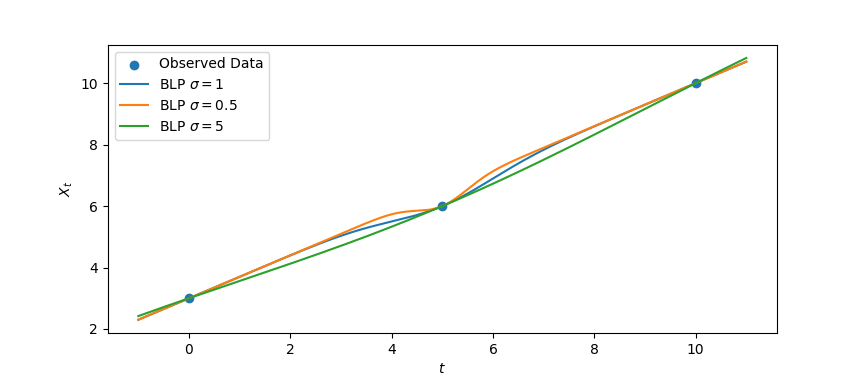
\includegraphics[width=\linewidth,keepaspectratio=true]{Figs/linearReversion.png}
				\caption{As with Fig. \ref{F:MeanRevert}, but with a linear transform ($g(t) = 0.7t + 3)$ applied.}\label{F:LinearRevert}
			\end{figure}

			Even with the smallest smoothing distance, we see that the prediction now reverts to a much more linear picture. Of course from a conceptual standpoint this is not a particularly attractive thing to have done -- one of the advantages of the BLP approach is that it is non-parametric, and we have essentially just added a layer of curve fitting on top. 

			However, we may think of the transform as essentially a prior on the functional form, which the observed data then updates. If we have sufficient data, then the predictor will ignore the prior -- as demonstrated in Fig. \ref{F:LinearPrior} where the prior is (intentionally) nothing like the true relationship. Aside from a few gaps in the data where the $\sigma = 0.5$ attempts to revert to the prior $g(t) = 0.7t + 3$, we see that the predictors are happy to ignore the prior in favour of the data, as we should expect.

			In interpreting the transform as a prior on the predictor, we see that it is therefore inappropriate for $g(t)$ to be determined based on the data -- the prior should be the knowledge of the predictor \textit{before} the data is gathered. Even in the simple (and very commonly used) case where $g(t) = \frac{1}{n} \vec{X} \cdot \mathds{1}_n$, i.e. the sample mean, this is `bootstrapping' the prior, which may lead to faulty conclusions.

			\begin{figure}
				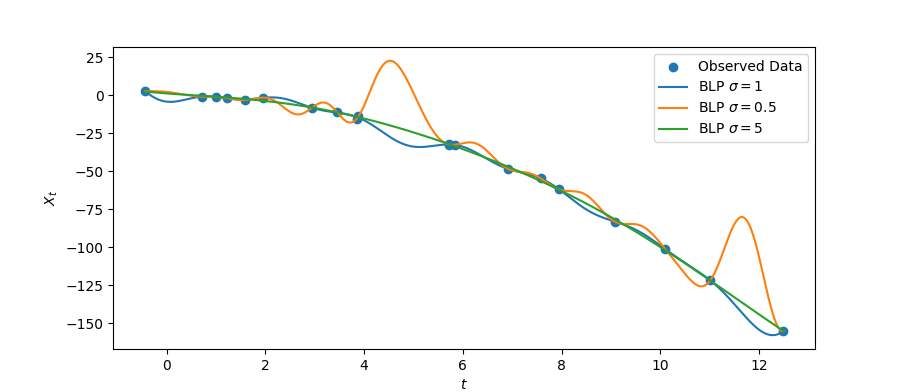
\includegraphics[width=\linewidth,keepaspectratio=true]{Figs/linearReversion_PriorExample.png}
				\caption{As with Fig. \ref{F:LinearRevert}, but where the data follows $X(t) = -t^2 + $noise, showing that the predictor can ignore the prior (which remains at $g(t) = 0.7t+3$) in the face of overwhelming data}\label{F:LinearPrior}
			\end{figure}
	\subsection*{Transforms on the Constrained Predictor}

		We now turn to the case of formalising the result of a constrained BLP --i.e. the BLMP -- using such a `Prior Transform'. This has an additional level of complexity because our constraint is on the untransformed data (i.e. $X_{t} \geq X_s$ if $t>s$), whilst the optimisation happens on the transformed data. We shall investigate if this results in any major discrepancies. 

		Using the same encodings as before ($\hat{X}_{t_i} = f_i(\vec{z})$), the Lagrangian becomes:

		\begin{spalign}
			\mathcal{L} = & \left(\sum_{i  = 0}^{N-1} \E{{X^\prime}_i^2} + \vec{a}_i \cdot K^\prime \vec{a}_i - 2 \vec{k}^\prime_i \cdot \vec{a}_i\right) - \mu_0 \left( \vec{a}_0\cdot\vec{X} + g(t_0)- z_0\right)
			\\ 
			&\quad - \sum_{i = 1}^{N-1} \mu_j \left(\left(\vec{a}_i - \vec{a}_{i-1}\right)\cdot \vec{X}^\prime - e^{z_i} + g(t_i) - g(t_{i-1}))\right)
		\end{spalign}
		Where again we have used $X^\prime_t = X_t - g(t)$, and $K^\prime$ and $\vec{k}^\prime$ are the second moment kernels on this transformed space. The optimal value of $\a$ in the t-BLMP are therefore identical to the solutions of the BLMP, with the addition of some primes:
		We then write:
		\begin{align}
			\ai^\prime & = \vi^\prime - \frac{\Delta_i}{2} \wi^\prime
			\\
			\vi^\prime & = {K^\prime}^{-1} \vec{k}^\prime_i
			\\
			\wi^\prime & = {K^\prime}^{-1} \vec{X}^\prime
		\end{align}
		Since $\ai \cdot \vec{X} = S_i - g(t_i)$, by definition, we therefore have:
		\begin{spalign}
			S_i & = A_i^\prime - \frac{\Delta_i}{2} B^\prime + g(t_i)
			\\
			A^\prime_i & = \vi \cdot \vec{X}^\prime
			\\
			B^\prime & = \wi^\prime \cdot \vec{X}^\prime
		\end{spalign}
		Therefore, we find that:
		\begin{equation}
			\vec{a}_i^\prime= \vi^\prime + \frac{S_i - A_i^\prime - g(t_i)}{B^\prime} \wi^\prime
		\end{equation}
		And hence:
		\begin{equation}
			\mathcal{L}(\vec{z}) = \text{const} + \sum_i S_i (S_i - 2(A^\prime_i + g(t_i))) \label{E:GeneralOptim}
		\end{equation}
		Hence:
		\begin{spalign}
			\pdiv{\mathcal{L}}{z_0} & = \frac{2}{B}\sum_{j=0}^{N-1}\left(S_j - (A_j + g(t_j))\right)
			%  \times \begin{cases}
			% 	1 & i = 0
			% 	 \\
			% 	e^{z_j} & 0 < j \leq N-1
			% \end{cases}
			\\
			\pdiv{\mathcal{L}}{z_{i>0}} & = \frac{2}{B}e^{z_i} \sum_{j=i}^{N-1}\left(S_j - (A_j + g(t_j)) \right)
		\end{spalign}

	\attempt{A General Formulation}

		We note that the formulation of \eref{E:GeneralOptim} is seems like it might be general, insofar as it does not (yet) contain any constraints - it is simply a reparameterisation of the Lagrangian in terms of the prediction values ($S_i$), the kernel and the sampeled data. As we shall see, it's not \textit{quite} general -- but almost. 

		It is worth recalling why this is useful - since it might appear that we have gone a roundabout way of computing things, given that the prediction values $(\hat{X}_t)$ appeared in the \textit{original} formulation, before we even introduced the kernel.

		The reason that the standard BLP formalism uses $\a$, $K$ and $\vec{k}_t$ is because they allow us to rewrite the Lagrangian in terms of these known terms, whilst relegating the uncomputable terms (namely $\llangle X_t \rrangle$) into a constant term. Since Lagrangians are invariant under the addition of total derivatives (and therefore constant terms), this has no impact on finding the optimal value of $\vec{a}$ -- we therefore neatly sidestep the inaccesible terms, by being willing to make an \textit{ansatz} about the form of $K$ and -- in the transformed version -- $g(t)$.

		This methodology therefore makes $\mathcal{L}$ computable - however it is now written in terms of $\a$, instead of $\hat{X}_t$. If we wish to impose conditions on $\hat{X}_t$, this is obviously less than desirable -- so we might wish to transform \textit{back} into $\hat{X}_t$ space (which we write as $S_i = \hat{X}_{t_i}$ for convenience). If $\a$ were a scalar, this would be a simple matter of writing $\ai = S_i/X_i$, but the dot product is non-invertible.

		The entire rigmarole above, therefore, amounts to finding a way to rewrite $\a$ as a function of $S_i$, which then allows us to write $\mathcal{L}$ as a function only of $S_i$, $K$ and $\vec{k}_t$. This can then be optimised over $\{S_i\}$, hence finding a general optimum -- of course, if $S_i$ is unconstrained then we recover $S_i = A_i + g(t_i)$, the standard BLP solution. 

		\subsubsection*{A General Proof}

			The above statement makes the claim that \eref{E:GeneralOptim} is a general result - however, the formulation of the Lagrangian is explicitly that of the monotonic predictor. We therefore produce a general result, which should make this evident\dots

			We begin, as before, with the standard BLP Lagrangian, with a sum over $i$ assumed to index into the $N$ prediction points $t_i \in T$:
			\begin{spalign}
				\mathcal{L}(\{\ai\}|\vec{X},k) = \left(\sum_{i  = 0}^{N-1} \E{{X^\prime}_i^2} + \vec{a}_i \cdot K^\prime \vec{a}_i - 2 \vec{k}^\prime_i \cdot \vec{a}_i\right) - \sum_j \lambda_j h_j(\{S\})
			\end{spalign}
			Here $h_j(\{S\})$ is the $j^\text{th}$ constraint on the final prediction values ($S_i = \hat{X}_{t_i} = g(t_i) + \ai \cdot \vec{X}^\prime$), such that $h_j(\{S\}) = 0$ if and only if the constraint is obeyed. We make the additional restriction that $h_j$ must be a \textit{linear} constraint, such that it can be written in the form:
			\begin{spalign}
				h_j = A - \sum_k b_{jk} S_k
			\end{spalign}
			Under this assumption, we can clearly see that:
			\begin{spalign}
				\pdiv{h_j}{\ai} & = \sum_m \pdiv{h_j}{S_m} \pdiv{S_m}{\ai}
				\\
				& = -b_{ji} \vec{X}^\prime
			\end{spalign}

			Therefore,
			\begin{spalign}
				\pdiv{L}{\ai} & = 2 K^\prime \ai - 2 \vec{k}^\prime_i + \underbrace{\left(\sum_j \lambda_j b_{ji} \right)}_{\eta_i} \vec{X}^\prime
				\\
				~
				\\
				& = 2 K^\prime \ai - 2 \vec{k}^\prime_i + \eta_i \vec{X}^\prime
			\end{spalign}
			Since $\eta_i$ is a function only of the Lagrange multipliers and the (constant) constraint terms, it is a constant in terms of $\ai$, and so:
			\begin{spalign}
				\pdiv{L}{\ai} = 0 \LLR \ai & = {K^\prime}^{-1} \left( \vec{k}^\prime - \frac{\eta_i}{2} \vec{X}^\prime \right)
				\\
				& = \vec{v}_i^\prime - \frac{\eta_i}{2} \wi^\prime
			\end{spalign}
			We can then impose our constraint that $S_i = g(t_i) + \ai \cdot \vec{X}$ to recover:
			\begin{spalign}
				\ai = \vi^\prime + \frac{S_i - A_i^\prime - g(t_i)}{B^\prime}
			\end{spalign}
			This is the exact result we had before, but written in the case of a much more general linear constraint. 

			We therefore have:
			\begin{spalign}
				\mathcal{L}= f(X_t,\vec{X}|k,T) + \frac{1}{B^\prime} \sum_i S_i\left(S_i - 2\left[A_i^\prime + g(t_i)\right] \right) - \sum_j \lambda_j h_j(\{S\})
			\end{spalign}

			We now make the assumption that $\{S\}$ is parameterised through another vector, $\vec{z}$ such that:
			\begin{spalign}
				S_i & = \mathcal{T}_i(\vec{z})
				\\
				h_j \left( \left\{ \mathcal{T}_i(\vec{z}) \right\} \right) & = 0 ~~\forall~j,i
			\end{spalign}
			I.e., $\mathcal{T}$ is a transform which guarantees all of the constraints are met, meaning that $\vec{z}$ is an unconstrained vector. The Lagrangian can now be written in terms of this unconstrained vector, giving the function to be optimised as (after some optimum-preserving rescaling):

			\begin{equation}
				\mathcal{L}^\prime(\vec{z} | \mathcal{T},\vec{X},k) = \sum_i \mathcal{T}_i(\vec{z}) \left( \mathcal{T}_i(\vec{z}) - 2 \big[ \vec{X}^\prime \cdot {K^\prime}^{-1} \vec{k}_i^\prime + g(t_i) \big] \right)
			\end{equation}

			The derivative of this function is:
			\begin{spalign}
				\pdiv{\mathcal{L}^\prime}{z_m}(\vec{z}) & = \sum_i 2 \left( \mathcal{T}_i(\vec{z}) - \big[ \vec{X}^\prime \cdot {K^\prime}^{-1} \vec{k}_i^\prime + g(t_i) \big] \right) \left. \pdiv{\mathcal{T}_i}{z_m} \right|_{\vec{z}}
				\\
				& = 2 \sum_i  \left( \mathcal{T}_i(\vec{z}) - Q_i \right) \left. \pdiv{\mathcal{T}_i}{z_m} \right|_{\vec{z}}
			\end{spalign}

			\subsection*{Some Examples}

				\subsubsection*{The Trivial Case: BLP}

					The simplest case the unconstrained case, with a suitable transform being $\mathcal{T}_i(\vec{z}) = z_i$. The derivative therefore simplifies to:
					\begin{spalign}
						\pdiv{\mathcal{L}^\prime}{z_m}(\vec{z}) & =\sum_i 2 \left( z_i- Q_i \right) \delta_{im}
						\\
						& = z_m - Q_i
					\end{spalign}
					Hence, the optimum lies at:
					\begin{spalign}
						z_m & =  g(t_m) +  \vec{k}_m^\prime \cdot \left({K^\prime}^{-1} \left(\vec{X} - \vec{G}\right) \right)
					\end{spalign}
					This is precisely the BLP case.

				\subsubsection*{The Monotonic Case: BLMP}
					\newcommand\T[1][i]{\mathcal{T}_{#1}}
					In the monotonic case, we write our transform as:
					\begin{spalign}
						\mathcal{T}_i(\vec{z}) = \begin{cases}
							z_0 & i = 0
							\\
							\mathcal{T}_{i-1}(\vec{z}) + e^{z_i} & \text{else}
						\end{cases}
					\end{spalign}
					Which gives the derivative:
					\begin{spalign}
						\pdiv{\T}{z_m} = \begin{cases} 
							1 & \text{ if } m = 0 
							\\
							e^{z_m} & \text{ if } 0 < m \leq i
							\\
							0 & \text{else}
						\end{cases}
					\end{spalign}
					This recovers the result we saw above. 

				\subsubsection*{The Normed Case: BLNP}

					A new case we might consider is the case were $\sum_i w_i S_i = C$, as might be the case if our function was constrained to have a certain integral value. In this case $w_i$ act as the weights of each abscissa, for which many algorithms exist -- we stick with a naive case of $w_i = \Delta t = \text{const}$, and write $C^\prime = C/\Delta t$.

					In this case, a suitable transform would be:
					\begin{equation}
						\T(\vec{z}) = \begin{cases} \frac{C^\prime}{1 + \sum_m e^{z_m}} & i = 0
							\\
							\frac{C^\prime e^{z_i}}{1 + \sum_m e^{z_m}} & \text{else}
						\end{cases}
					\end{equation}
					Note that the dimensionality of the problem has been reduced - $\vec{z}$ has dimensions $N-1$, since this is an equality constraint. This has derivatives
					\begin{spalign}
						\pdiv{\T}{z_m} = \delta_{im} \T - \frac{1}{C^\prime} \T[m] \T
					\end{spalign}
					Therefore the Lagrangian derivative is:
					\begin{spalign}
						\pdiv{\mathcal{L}^\prime}{z_m}(\vec{z}) & = 2 \sum_i \left( \mathcal{T}_i(\vec{z}) - Q_i\right) \left. \pdiv{\mathcal{T}_i}{z_m} \right|_{\vec{z}}
						\\
						& = 2 \T[m] \left[ \left( \T[m] - Q_m \right) - \frac{1}{C^\prime} \sum_i \T[i] \left( \T - Q_i\right) \right]
					\end{spalign}
				
				\subsubsection*{The Tightly Bounded Predictor: BLBP}
					
					Consider now the case where the predictor values are tightly bounded, such that $C \leq S_i \leq D \forall i$. A suitable encoding might be:
					\begin{spalign}
						\T(\vec{z}) = \frac{D + C e^{-z_i}}{1 + e^{-z_i}} 
					\end{spalign}
					Hence:
					\begin{spalign}
						\pdiv{\T}{z_m} & = (D - C) \frac{e^{-z_m}}{(1 + e^{-z_m})^2} \delta_{im}
						\\
						~
						\\
						\pdiv{L}{z_m} &= 2(D-C) \left(\T[m] - Q_m\right) \frac{(\T[m] - C_m)(D-\T[m])}{D^2}
					\end{spalign}
					Perhaps logically, we see once again that this has solutions:
					\begin{equation}
						\T[m] = \begin{cases}
							Q_m & \text{if } C \leq Q_m \leq D
							\\
							C  & \text{if } Q_m < C
							\\
							D & \text{if } Q_m > D
						\end{cases}
					\end{equation}
					Recalling that $\T[m] = Q_m$ is the BLP solution, we see that the Best-Linear-Bounded-Predictor simplifies trivially to the BLP subject to a floor-and-ceiling truncation.
\end{document}